\chapter{Methodology}
\section{Time to Digital Converter}

\subsection{specifications}
The main specifications for the TDC are the following:
\begin{itemize}
    \item Corner set up: TT, 60$^{\circ}$C, 1.2 V.
    \item Static phase error ($\Delta_t$) < 1\%.
    \item Clock reference frequency: 100 MHz.
    \item Number of bits: 4.
    \item Acquisition range (dynamic range): -2$\pi$ to 2$\pi$.
\end{itemize}

The TDC implements a 4-bit flash architecture for a time resolution of 625 ps ($\Delta$) in each half of the clock period. The acquisition range is 20 ns, which corresponds to a phase 
range of -2$\pi$ to 2$\pi$ for a clock frequency of 100 MHz.

\subsection{Architecture}
The TDC architecture is based on the bipolar TDC presented in \cite{Henzler2010}. The core of the TDC consist of a voltage-controlled delay line (VCDL), a set of D flip-flops to sample the
state of the VCDL, and a thermometer-to-binary decoder that process the sampled data to produce a workable digital output. This arrangement is used twice, once for the case when the
feedback signal has a lower frequency (or delayed phase) than the reference clock, and the other for the case when the feedback signal has a higher frequency (or advanced phase) than
the reference clock. The two outputs are then combined to produce the final output of the TDC. Such an architecture (Fig. \ref{fig:TDC_conventional_architecture}) would be the 
conventional way to implement a TDC that reads both cases for the phase difference between the reference clock and the feedback signal. 

\begin{figure}[h]
    \centering
    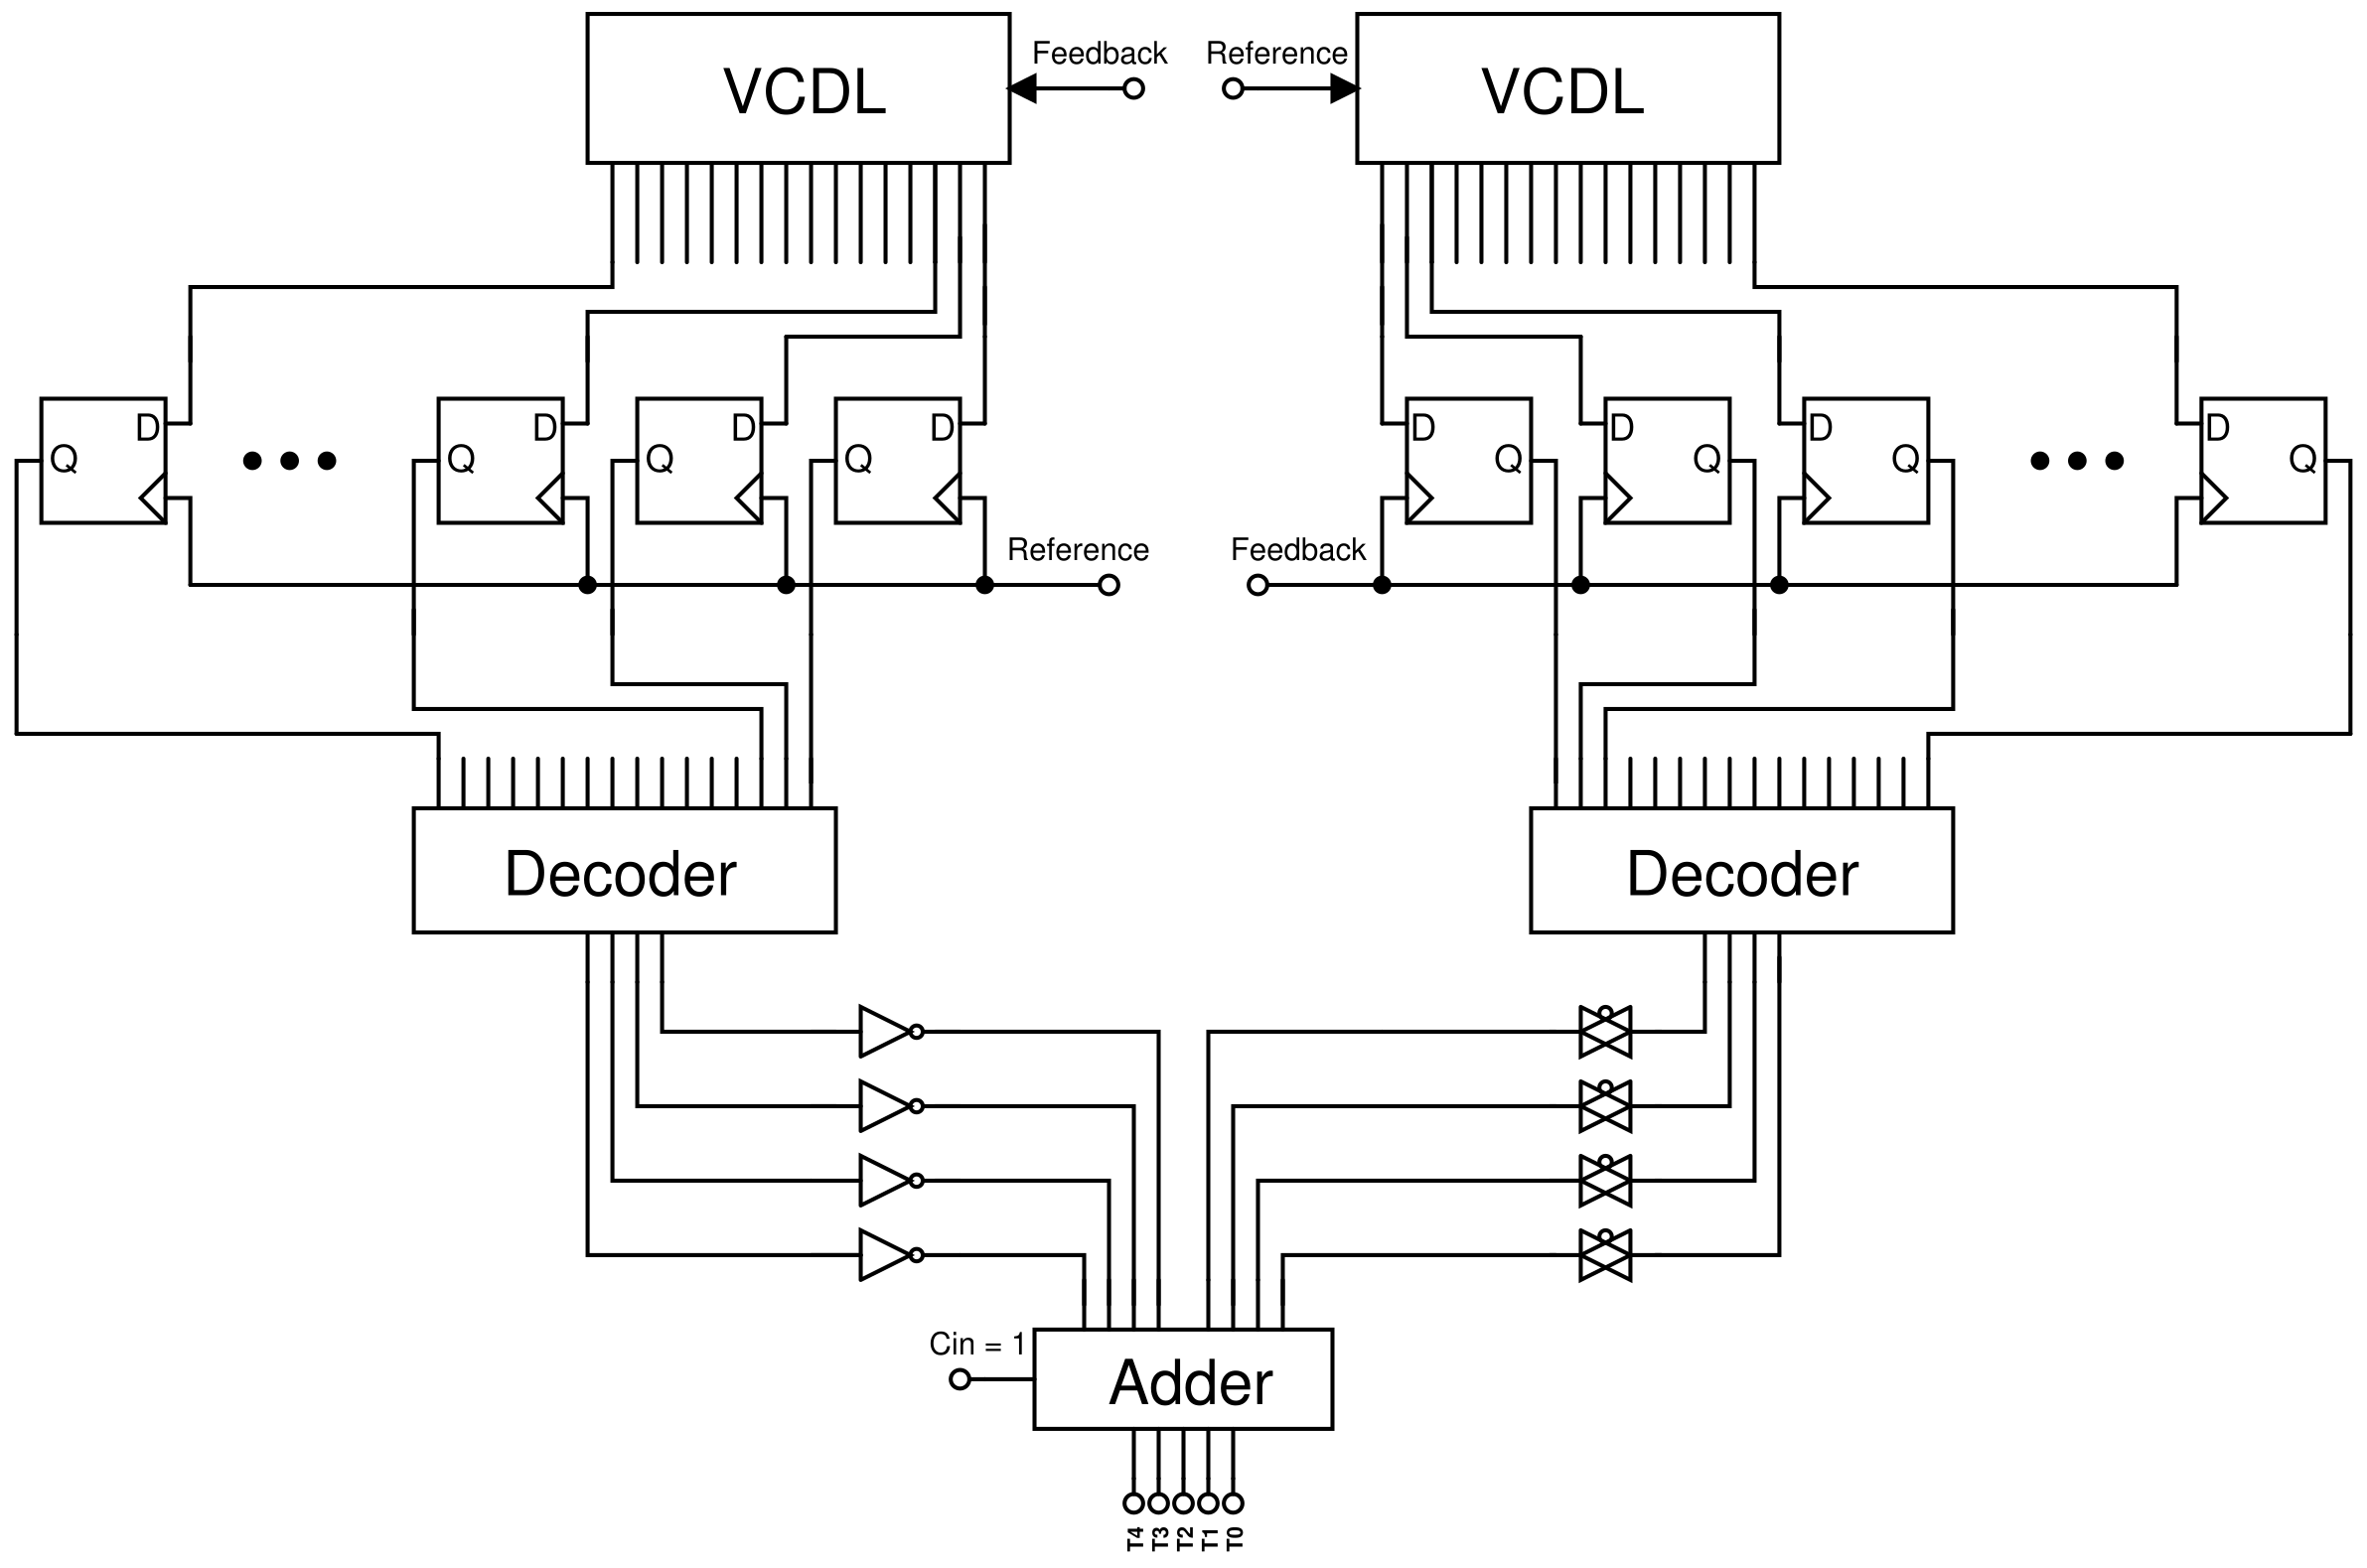
\includegraphics[width=1\textwidth]{figures/TDC_conventional_architecture.png}
    \caption{Conventional bipolar TDC architecture}
    \label{fig:TDC_conventional_architecture}
\end{figure}

The architecture of figure \ref{fig:TDC_conventional_architecture} has shortcomings, such as the fact that it does not allow for a phase difference of more than 2$\pi$ between the
reference clock and the feedback signal, meaning that the TDC will not be able to read the phase difference beyond half cycle for each clock period. This is limiting for the PLL, as it
would not be able to correct the phase difference if it exceeds $\pi$ for each case. To overcome this limitation and achieve the desired acquisition range set in the specifications, 
the TDC architecture of figure \ref{fig:TDC_proposed_architecture} is proposed.

\begin{figure}[h]
    \centering
    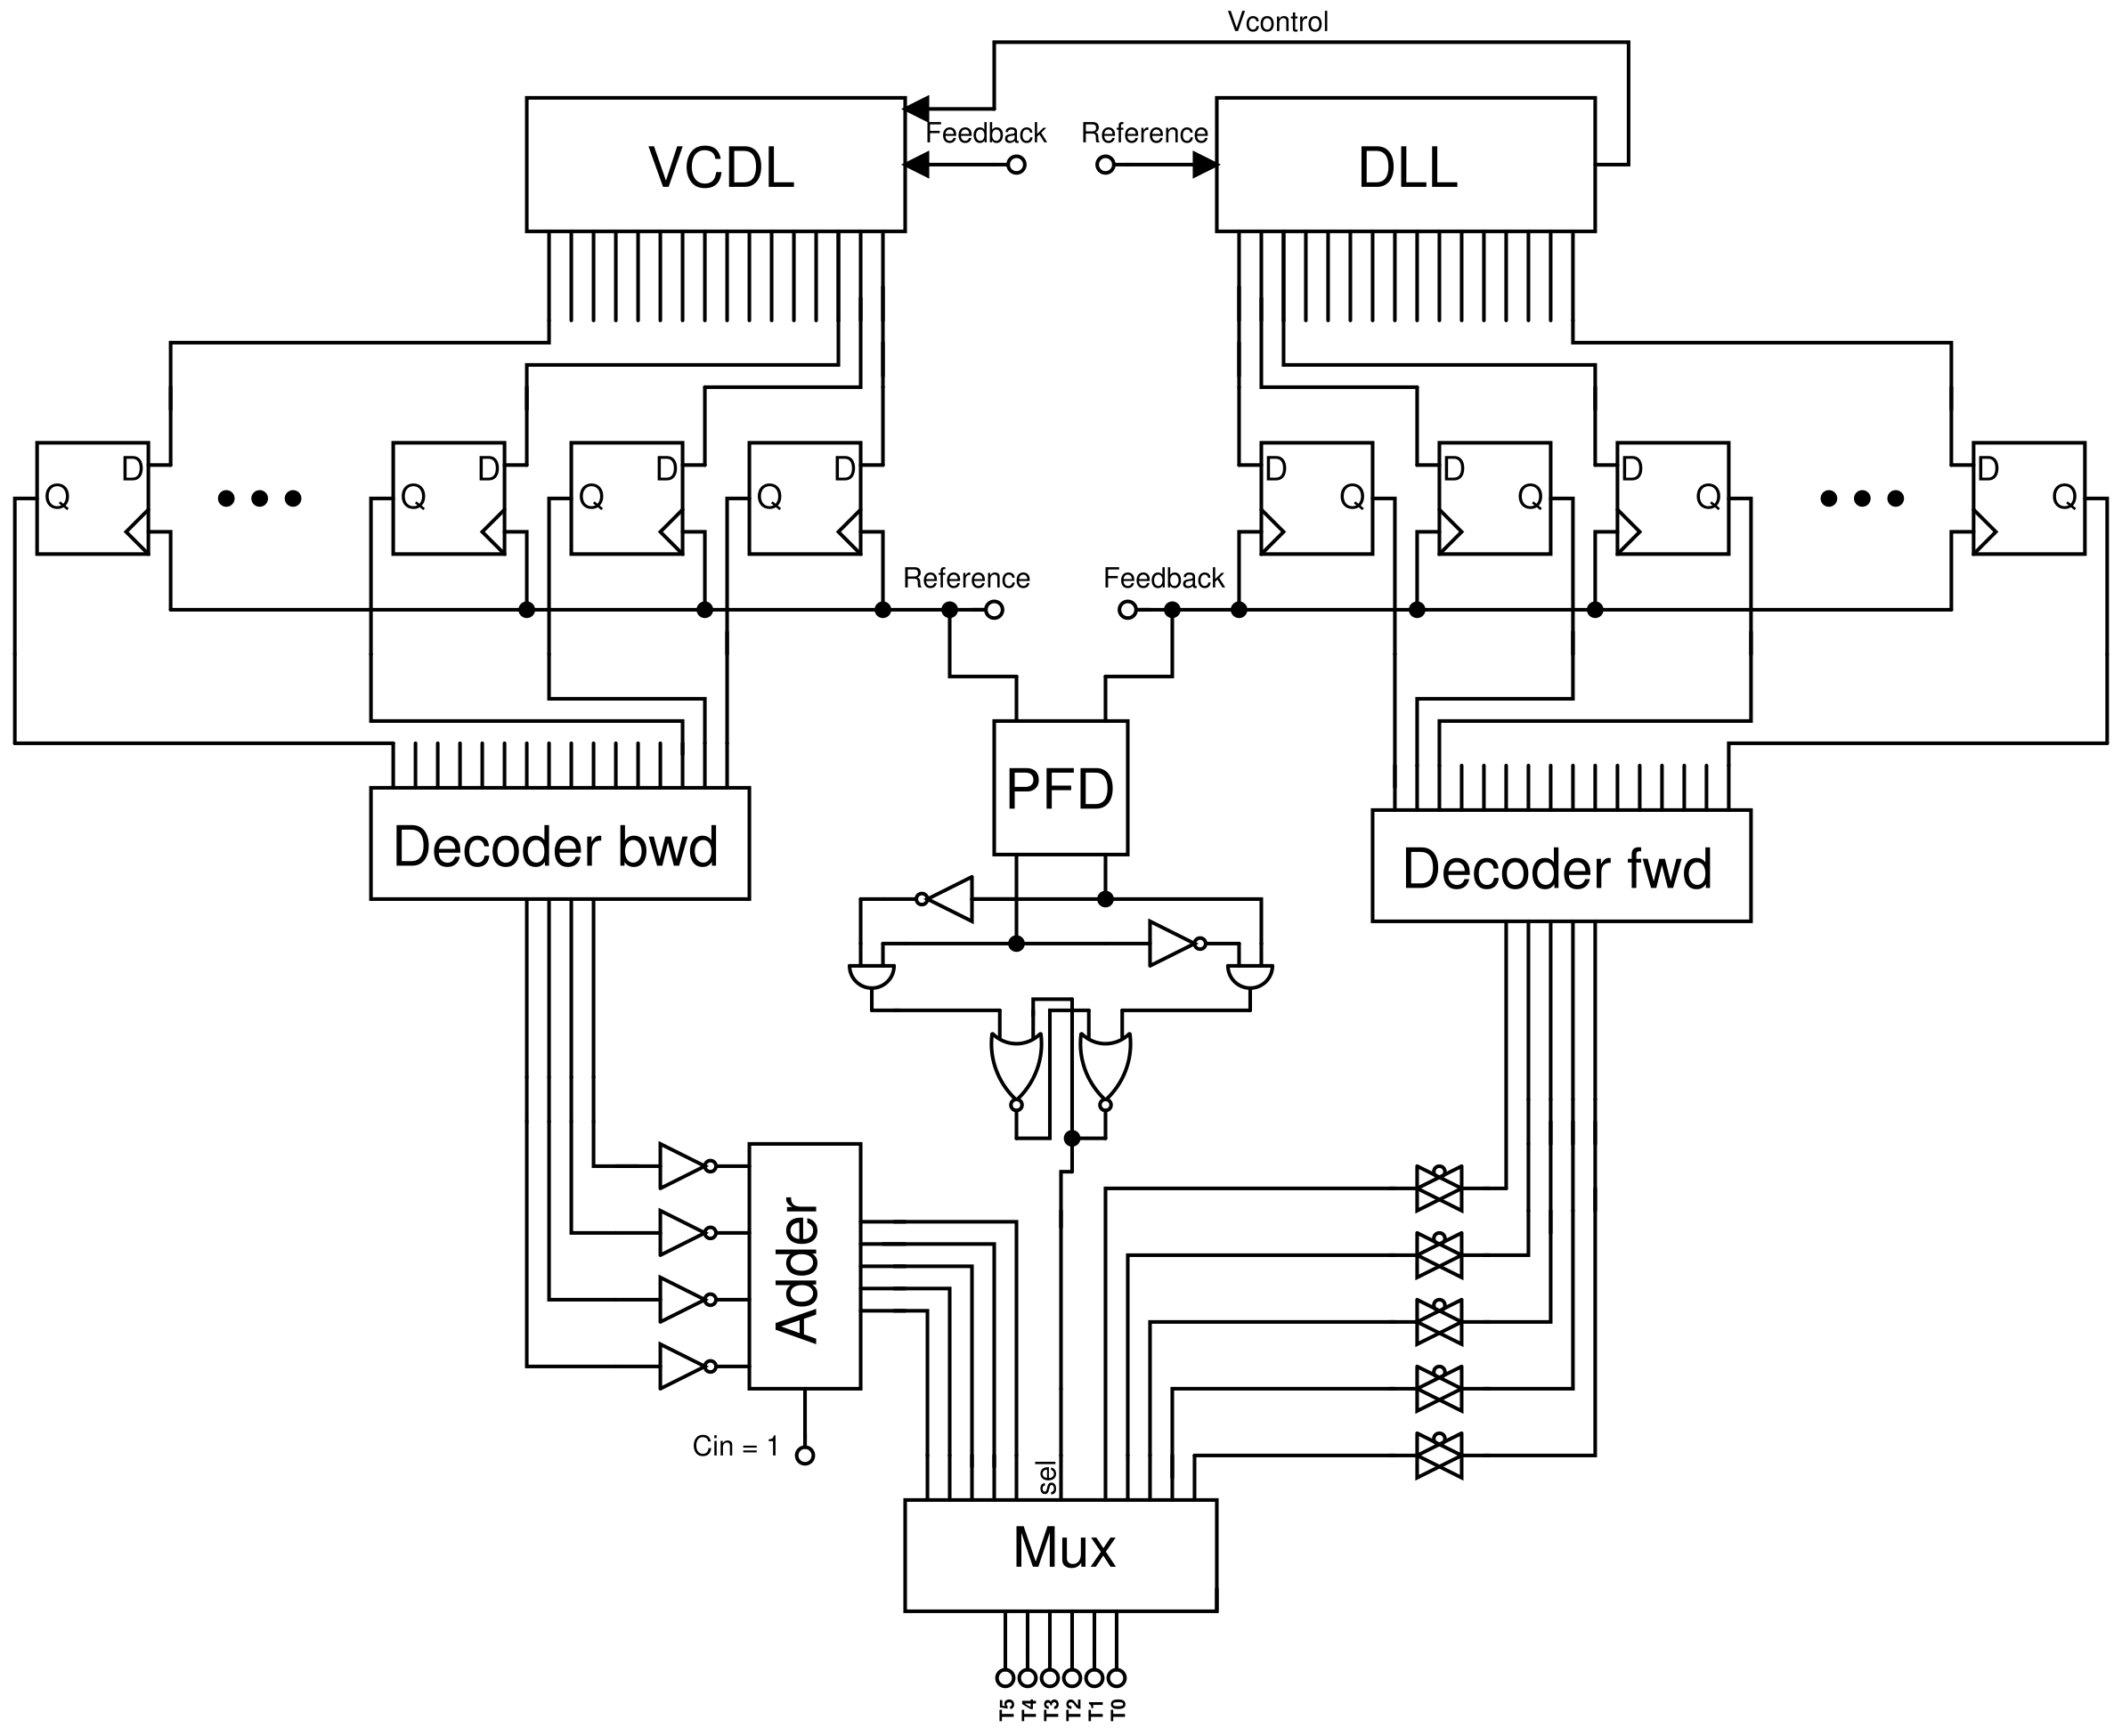
\includegraphics[width=1\textwidth]{figures/TDC_proposed_architecture.png}
    \caption{Proposed bipolar TDC architecture}
    \label{fig:TDC_proposed_architecture}
\end{figure}

The main differences between the conventional bipolar architecture and the proposed one are that the latter uses a DLL instead of a VCDL to implement the delay line, a slight modification
to the thermometer-to-binary decoder, and a different way to combine the outputs of the two TDCs.

The DLL allows for a more robust and stable delay line as it is less sensitive to PVT variations. This is important for the PLL, as it needs to be able to operate under different
conditions and still be able to correct the phase difference between the reference clock and the feedback signal.

The thermometer-to-binary decoder is modified to allow for the reading of both cases of the phase/frequency difference between the signals. This is the main way that the proposed bipolar TDC is able
to read a phase difference of more than 2$\pi$ each cycle and as far as the author is aware, this is the first time that such a modification has been proposed in the literature.

Finally, the outputs of the two TDCs are combined using a multiplexer that selects the output based on the frequency state of the feedback signal. The selector needs to be able to
determine whether the feedback signal is leading or lagging the reference clock, which is done by retrieving the information lost because of the decoder modification.


All of this modifications achieve a 5-bit bipolar TDC with no zero-gain region using just two 4-bit delay line TDCs. Such changes done to the conventional bipolar TDC architecture will be further 
explained in the following sections of this chapter, where the design of the TDC will be presented in detail.

\subsection{System behavior}
Both architectures have the same principle of operation and each of their blocks have the same behavior. Both architectures have some sort of delay line that measures the phase difference
between the reference clock and the feedback signal, a thermometer-to-binary decoder that processes the sampled data to produce a workable digital output, and both have the same number of 
D flip-flops to sample the state of the delay line which is equal to $2^n$ where $n$ is the number of bits of the TDC.

The operation of the TDC of \ref{fig:TDC_conventional_architecture} is as follows: When the rising edge of the reference clock occurs and a new cycle starts, the circuit in charge of reading the 
case where the feedback signal is lagging (forward) with respect to the reference will start its operation, meaning that its VCDL will be reset and start counting the delay until the next rising 
edge of either the reference clock or the feedback signal occurs. If the former occurs first, then the circuit in charge of reading the case where the feedback signal is leading (backward) will 
never start its operation and the TDC output will be the same as the last cycle. If the latter occurs first, then the backward circuit will start its operation and count the remaining delay until
the next rising edge of the reference clock and the TDC output will be the subtraction of the forward output minus the backward output.

Because the decoders of the TDC of figure \ref{fig:TDC_conventional_architecture} are thermometer-to-binary decoders, their output is equal to 0 after half of the reference clock period time has
passed, meaning the result of the TDC will be either the forward output or the 2's complement of the backward output depending on which of the half cycle of the clock period the feedback signal
occurs. This feature is what allows the TDC to detect whether the feedback signal is leading or lagging the reference clock, but it is also what limits the TDC to a phase difference of $\pm \pi$
each cycle.

\begin{figure}[H]
    \centering
    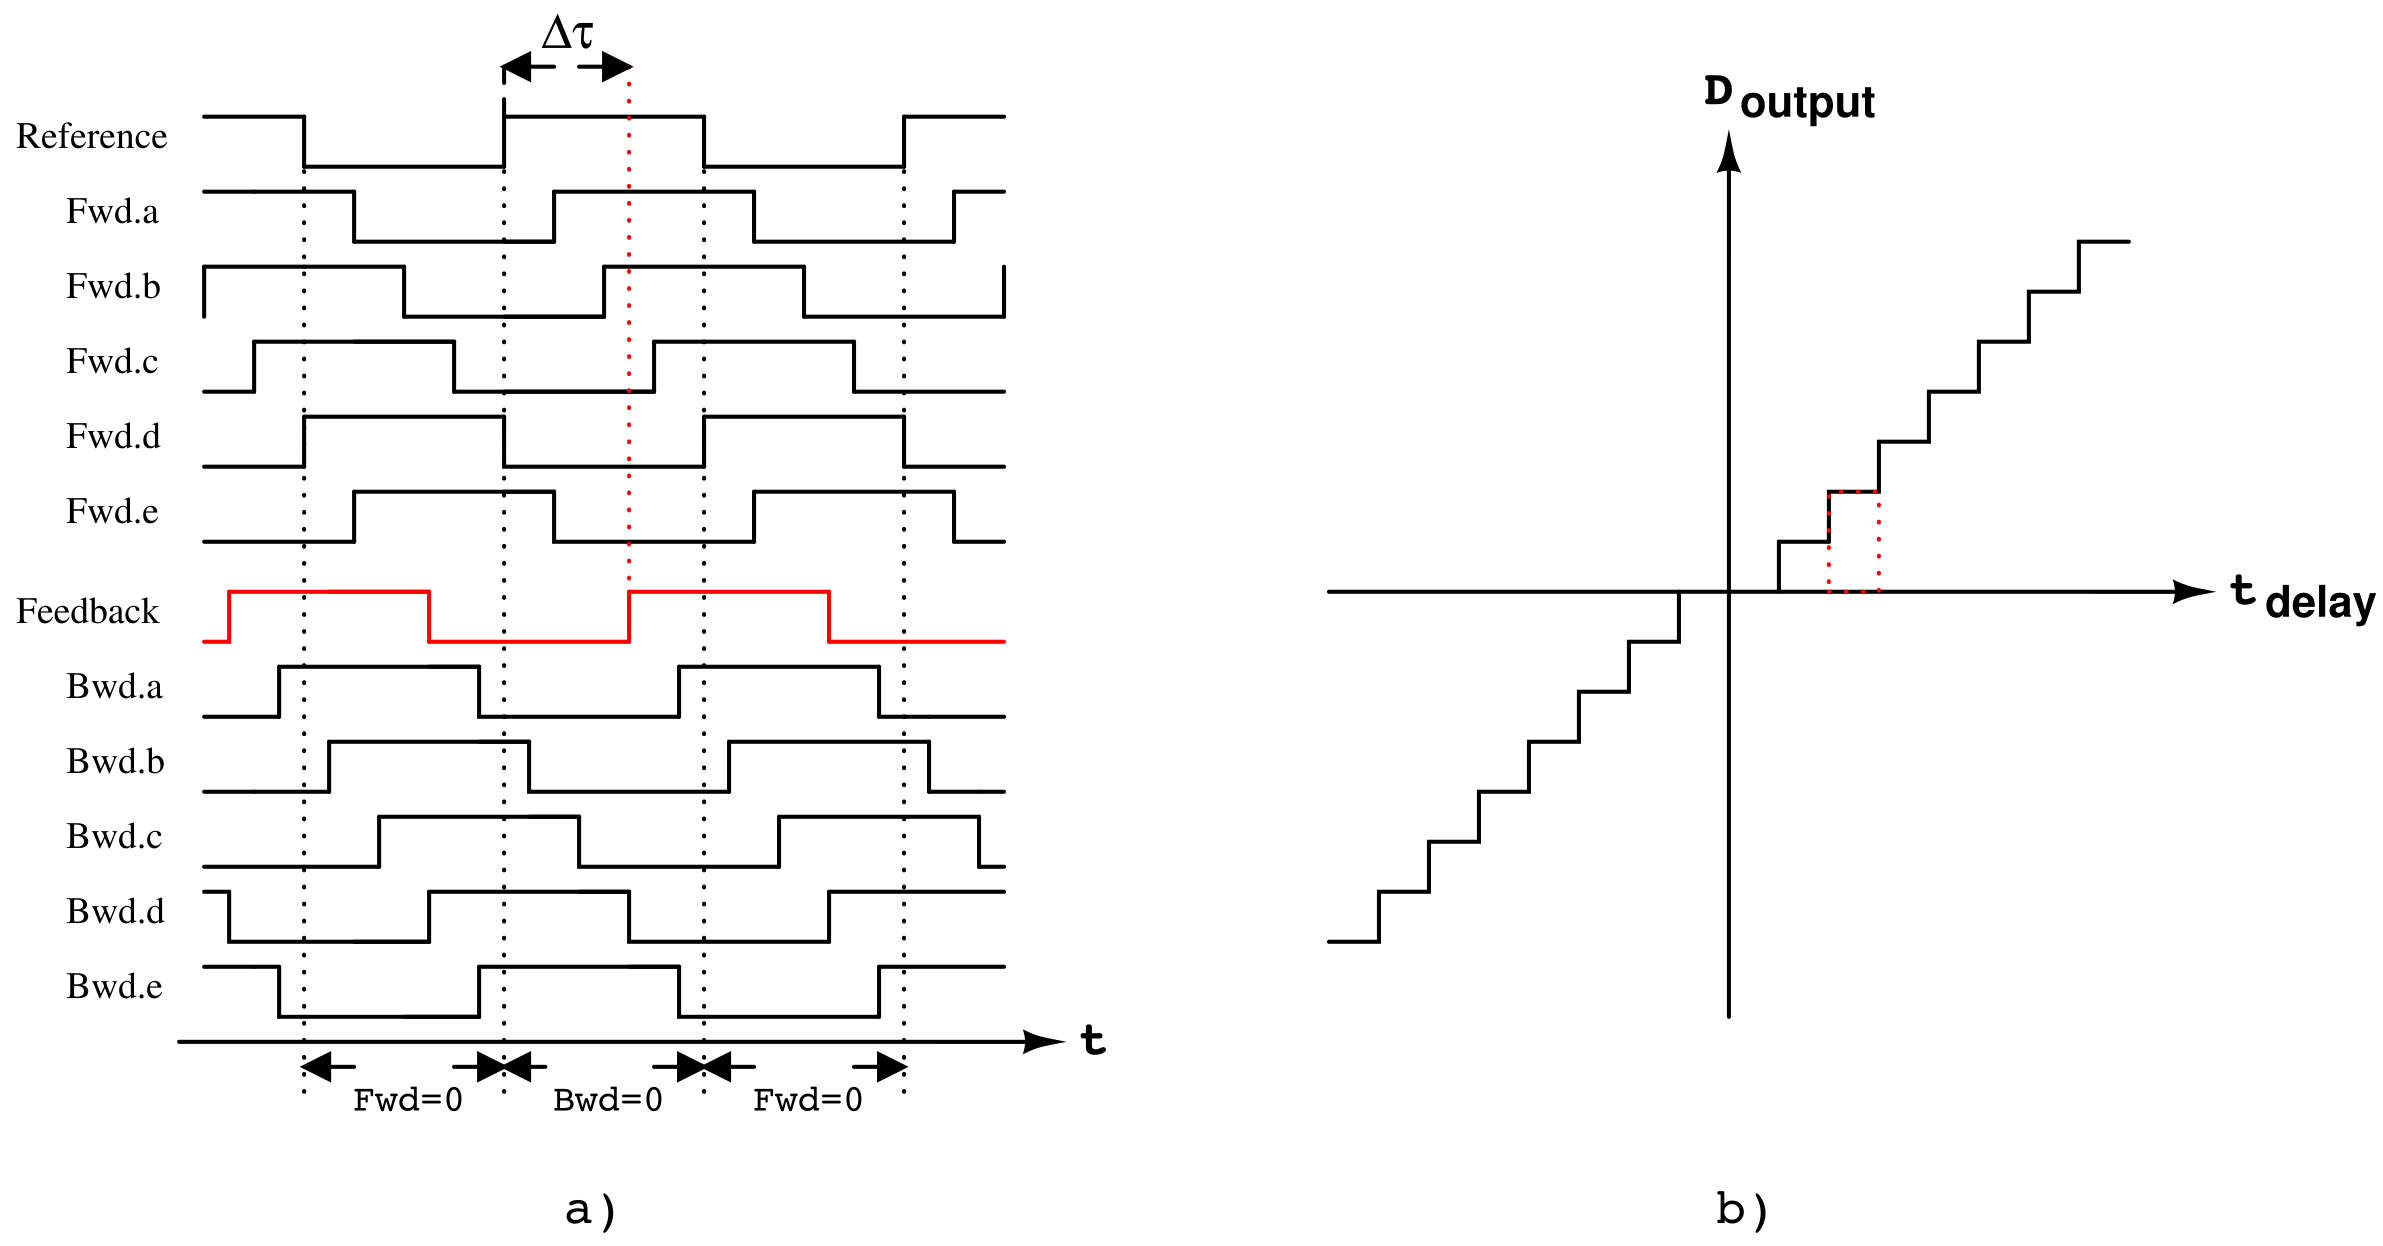
\includegraphics[width=1\textwidth]{figures/TDC_timing_diagram.png}
    \caption{a) Conventional bipolar TDC timing diagram for a positive phase error, and b) its ideal characteristic.}
    \label{fig:TDC_conventional_timing_diagram}
\end{figure}

Figure \ref{fig:TDC_conventional_timing_diagram} further elaborates on this point, showing the timing diagram and the ideal characteristic of the conventional bipolar architecture. Notice that there 
is a 0 gain zone around zero delay where the TDC will not be able to detect small phase differences, also notice that the output will only take values between 7 and -7 for a 4-bit TDC. Both of
these issues are addressed in the proposed architecture.

\subsection{Design}
The design for the TDC proposed in this work is approached in a modular way, where each block is designed separately and then integrated into the final TDC. Even though differences exist between
both paths (forward and backward) of the TDC, the blocks are the exact same for both, meaning that the design can be done in a single step and then replicated for each path with
slight modifications.

\subsubsection{DLL}
The implementation of the DLL is that of figure \ref{fig:DLL_architecture}, which is based on \cite{Razavi_DLL_article}. The DLL is composed of a voltage-controlled delay line (VCDL) that is used
to measure the phase difference between the reference clock and the feedback signal, a charge pump that is used to control the delay of the VCDL, and a phase frequency detector (PFD) that is used to
determine whether the feedback signal is leading or lagging the reference clock.

\paragraph{VCDL}
The delay elements of the VCDL are implemented using a series of CMOS inverters whose delay is controlled by a variable resistor (MOSFET in triode region) at the source of the M1 (see Fig. \ref{fig:VCDL_delay_elements}).
Each one of this elements must have a delay equal to 625 ps for a total of 10 ns (the period of the reference clock) after 16 of them. 625 ps is a relatively high amount of delay for a CMOS inverter of
minimum dimensions in 65 nm, there are multiple approaches towards meeting such a high delay, but the preferable method from the perspective of optimizing the phase noise according to \cite{Razavi_PLL_book}
is to increase the number of stages.

\begin{figure}[H]
    \centering
    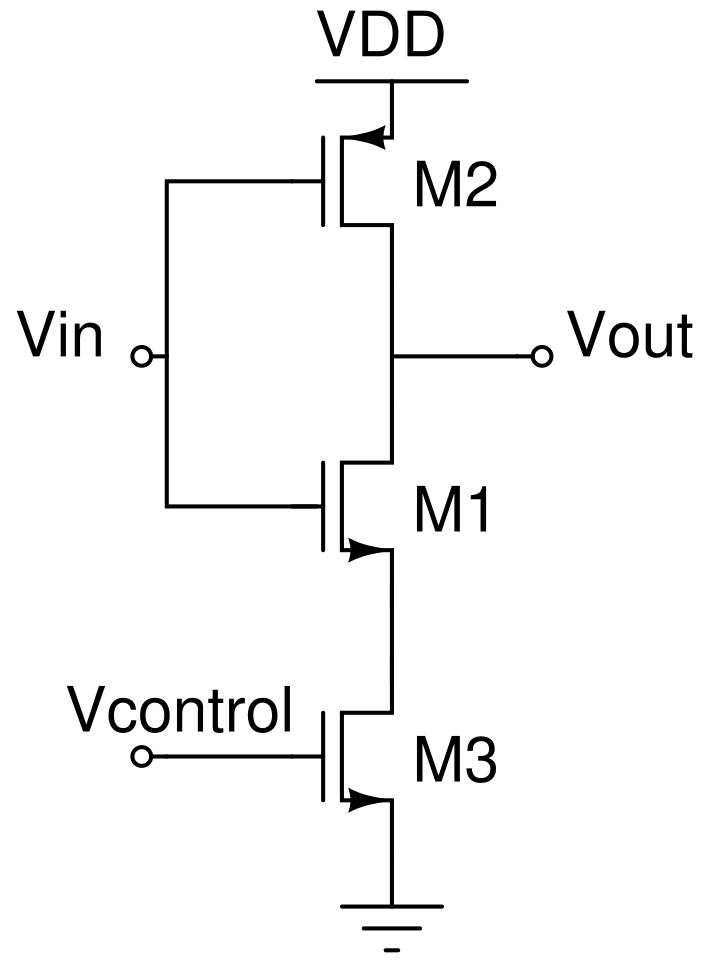
\includegraphics[width=0.35\textwidth]{figures/VCDL_element.png}
    \caption{CMOS inverter with a variable active resistor.}
    \label{fig:VCDL_delay_elements}
\end{figure}

Therefore after simulating the circuit of figure \ref{fig:VCDL_delay_elements} and measuring its delay (for a load of another identical inverter) it was determined that the number of stages necessary to achieve
625 ps in each delay element is 14. The dimensions for all 3 MOSFETs are annotated in table \ref{tab:VCDL_delay_elements_dimensions}. Notice that the inverter NMOS is wider than the PMOS
to compensate for the source degeneration of the NMOS.

\begin{table}[h]
    \centering
    \begin{tabular}{|c|c|c|}
        \hline
        \textbf{Transistor} & \textbf{Length ($\mu$m)} & \textbf{Width ($\mu$m)} \\
        \hline
        M1 & 0.06 & 0.215 \\
        M2 & 0.06 & 0.08 \\
        M3 & 0.3 & 0.3 \\
        \hline
    \end{tabular}
    \caption{Dimensions of the VCDL delay elements}
    \label{tab:VCDL_delay_elements_dimensions}
\end{table}

\paragraph{PFD}
The PFD implemented for the DLL is the one presented in \ref{fig;PFD_schematic}. The function of the PFD is to compare the phase and frequency of the reference clock and the feedback signal, and to generate
the appropriate control signals (UP and DOWN) for the charge pump. The resettable D flip-flops are implemented using the latches shown in figure \ref{fig:D_ff}, where the output of each latch
drives one input of the other.

The time it takes from the rising edge of the RESET signal to the point where both outputs (UP and DOWN) are low (T$_{res}$) is the dead zone of the PFD, which is a critical parameter as it determines the minimum
phase difference that the DLL can detect and it is equal to approximately 64.34 ps for the design presented in this work.


\noindent\begin{minipage}{0.48\textwidth}
    \begin{center}
        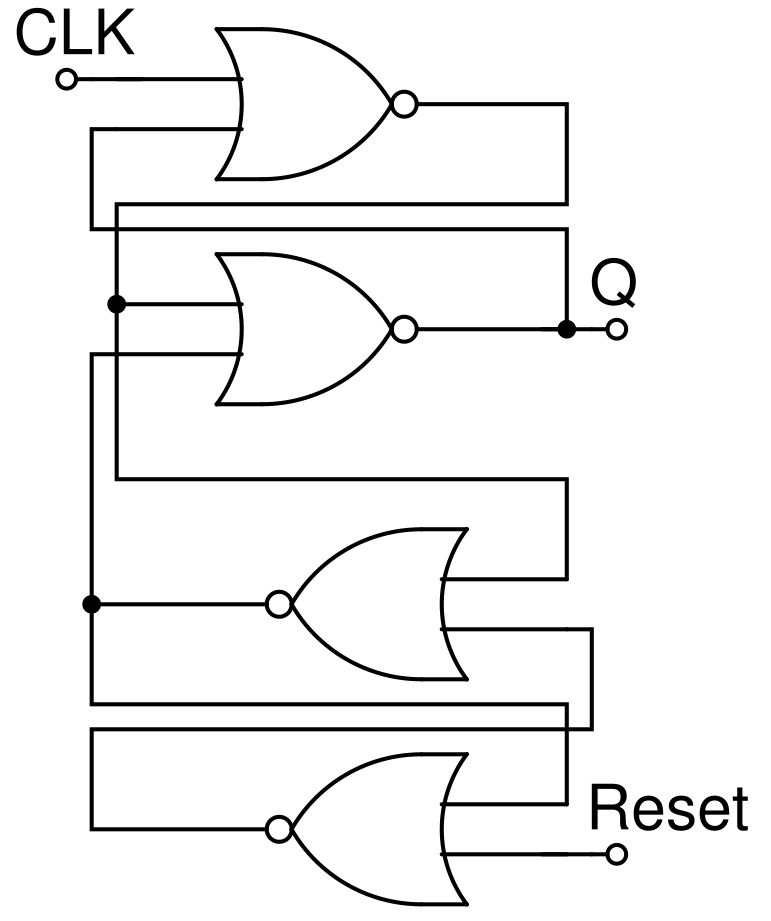
\includegraphics[width=0.72\textwidth]{figures/PFD_ff.png}
        \captionof{figure}{Simple resettable D flip-flop consisting of two cross-couped latches.}
        \label{fig:D_ff}
    \end{center}
\end{minipage}
\hspace{0.02\textwidth}
\begin{minipage}{0.48\textwidth}
\begin{center}
    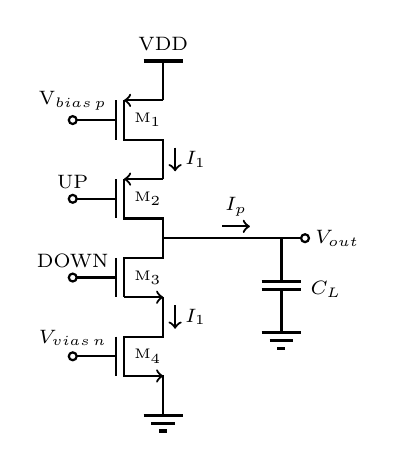
\begin{tikzpicture}
            \draw[very thick] (0,0) -- node[above]{\scriptsize VDD} (0.5,0);
            \draw[thick] (0.25,0) -- (0.25,-0.5);
            \draw[thick, ->] (0.25,-0.5) -- (-0.25,-0.5);
            \draw[thick] (-0.25,-0.5) -- node[right]{\tiny M$_1$} (-0.25,-1) -- (0.25,-1) -- (0.25,-1.5);
            \draw[thick, ->] (0.25,-1.5) -- (-0.25,-1.5);
            \draw[thick] (-0.25,-1.5) -- node[right]{\tiny M$_2$} (-0.25,-2) -- (0.25,-2) -- (0.25,-2.5) -- (-0.25,-2.5) -- node[right]{\tiny M$_3$} (-0.25,-3);
            \draw[thick, ->] (-0.25,-3) -- (0.25,-3);
            \draw[thick] (0.25,-3) -- (0.25,-3.5) -- (-0.25,-3.5) -- node[right]{\tiny M$_4$} (-0.25,-4) -- (0.25,-4) -- (0.25,-4.5);
            \draw[thick, ->] (-0.25,-4) -- (0.25,-4);
            \draw[very thick] (0,-4.5) -- (0.5,-4.5);
            \draw[very thick] (0.1,-4.6) -- (0.4,-4.6);
            \draw[very thick] (0.2,-4.7) -- (0.3,-4.7);
            
            \draw[thick, ->] (0.4,-1.1) -- node[right]{\scriptsize $I_1$} (0.4,-1.4);
            \draw[thick, ->] (0.4,-3.1) -- node[right]{\scriptsize $I_1$} (0.4,-3.4);
            \draw[thick] (-0.35,-0.5) -- (-0.35,-1);
            \draw[thick] (-0.35,-1.5) -- (-0.35,-2);
            \draw[thick] (-0.35,-2.5) -- (-0.35,-3);
            \draw[thick] (-0.35,-3.5) -- (-0.35,-4);
            \draw[thick] (-0.35,-0.75) -- (-0.85,-0.75);
            \draw[thick] (-0.35,-1.75) -- (-0.85,-1.75);
            \draw[thick] (-0.35,-2.75) -- (-0.85,-2.75);
            \draw[thick] (-0.35,-3.75) -- (-0.85,-3.75);
            \draw[thick] (-0.9,-0.75) circle (0.05) node[above] {\scriptsize V$_{bias \, p}$};
            \draw[thick] (-0.9,-1.75) circle (0.05) node[above] {\scriptsize UP};
            \draw[thick] (-0.9,-2.75) circle (0.05) node[above] {\scriptsize DOWN};
            \draw[thick] (-0.9,-3.75) circle (0.05) node[above] {\scriptsize $V_{vias \, n}$};

            \draw[thick] (0.25,-2.25) -- (2,-2.25);
            \draw[thick, ->] (1,-2.1) -- node[above]{\scriptsize $I_p$} (1.35,-2.1); 
            \draw[thick] (2.05,-2.25) circle (0.05) node[right] {\scriptsize $V_{out}$};
            \draw[thick] (1.75,-2.25) -- (1.75,-2.8);
            \draw[very thick] (1.5,-2.8) -- (2,-2.8);
            \draw[very thick] (1.5,-2.9) -- node[inner sep = 10, right]{\scriptsize $C_L$} (2,-2.9);
            \draw[thick] (1.75,-2.9) -- (1.75,-3.45);
            \draw[very thick] (1.5,-3.45) -- (2,-3.45);
            \draw[very thick] (1.6,-3.55) -- (1.9,-3.55);
            \draw[very thick] (1.7,-3.65) -- (1.8,-3.65);
    \end{tikzpicture}
\end{center}
\captionof{figure}{CMOS drain switched charge pump.}
\label{fig:CP_schematic_methodology}
\end{minipage}

\paragraph{Charge pump}
The charge pump implemented for the DLL is the drain switched CP described in chapter 2 and shown again in figure \ref{fig:CP_schematic_methodology}. As stated before, the most challenging
aspect of designing the CP is to minimize the current mismatch ($\Delta_I$) between both branches, the approach taken in this work towards achieving this goal is to use relatively long current sources
(M1 $\&$ M4) and low resistance switches (M2 $\&$ M3) to minimize the effect of the channel length modulation. 

The static phase error ($\Delta_t$) to which the DLL will lock onto is determined not only by ($\Delta_I$) but also by the nominal charge pump current ($I_p$) as described in
equation \ref{eq:steady_state_phase_error}. Hence, with the purpose of minimizing ($\Delta_t$) and making the TDC as accurate as possible, the current sources of the CP in 
figure \ref{fig:CP_schematic} are designed to have a current of 150 $\mu$A, which is a good compromise between the static phase error, the power consumption and the area of the CP.

The specifications set $\Delta_t$ percentage to be less than 1\%, which corresponds to a maximum $\Delta_I$ of 14.6 $\mu$A for a t$_{res}$ of 64.34 ps according to equation
\eqref{eq:steady_state_phase_error}. The designed dimensions that meet this requirements are shown in table \ref{tab:CP_dimensions}. All that is left is to design the loop filter,
which for the DLL it consist of a single capacitor (C$_L$) connected to the output of the CP. There is no need for a second order filter because the DLL doesn't have a VCO that 
contributes with a pole at the origin, making the choice of C$_L$ less critical than in a PLL \cite{Razavi_DLL_article}. The considerations for choosing C$_L$ are mainly the
stability of the loop and the locking time, for this design a value of 3 pF is chosen as it provides a good trade-off between both parameters.


\begin{table}[h]
    \centering
    \begin{tabular}{|c|c|c|}
        \hline
        \textbf{Transistor} & \textbf{Length ($\mu$m)} & \textbf{Width ($\mu$m)} \\
        \hline
        M1 & 0.3 & 3.6 \\
        M2 & 0.06 & 1.2 \\
        M3 & 0.06 & 1.2 \\
        M4 & 0.3 & 3.6 \\
        \hline
    \end{tabular}
    \caption{Dimensions of the charge pump transistors}
    \label{tab:CP_dimensions}
\end{table}

\subsubsection{Sampling flip-flops}
The sampling flip-flops are implemented using the same resettable D flip-flops shown in figure \ref{fig:D_ff}. The number of flip-flops used is equal to $2^n$ where n is the number of bits of the TDC,
which for this design is 16 (one extra flip-flop is added at the output of the last stage in order to have the same charge at the output of each stage of the VCDL). The flip-flops are connected 
in parallel and their clock input is driven by the feedback signal for the forward path and by the reference clock for the backward path. The reset input of all flip-flops is set to low because the control
is done at the multiplexer block, not at the flip-flops.

\subsubsection{modified thermometer-to-binary decoders}
The standard thermometer-to-binary decoder for a 4-bit flash TDC has the truth table shown in table \ref{tab:standard_decoder_truth_table}, where the inputs A-P are the outputs of the DLL sampled by the flip-flops.
Figure \ref{fig:DLL_output_TRAN} shows the timing diagram of the DLL output, here A is the output of the last stage of the delay line (when exactly 10 ns have passed since the rising edge of the reference clock)
and P is the reference clock itself (before the first stage of the delay line).

\begin{table}
    \centering
    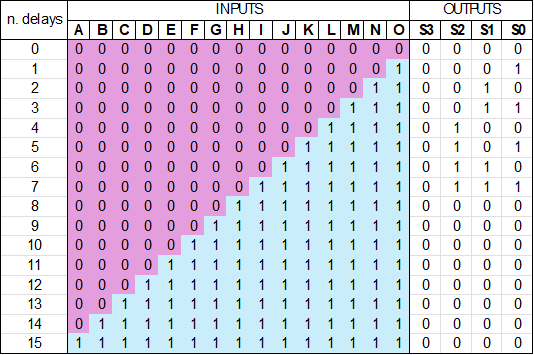
\includegraphics[width=0.7\textwidth]{figures/standard_decoder_truth_table.png}
    \caption{Truth table of the standard thermometer-to-binary decoder for a 4-bit TDC.}
    \label{tab:standard_decoder_truth_table}
\end{table}

\begin{figure}[H]
    \centering
    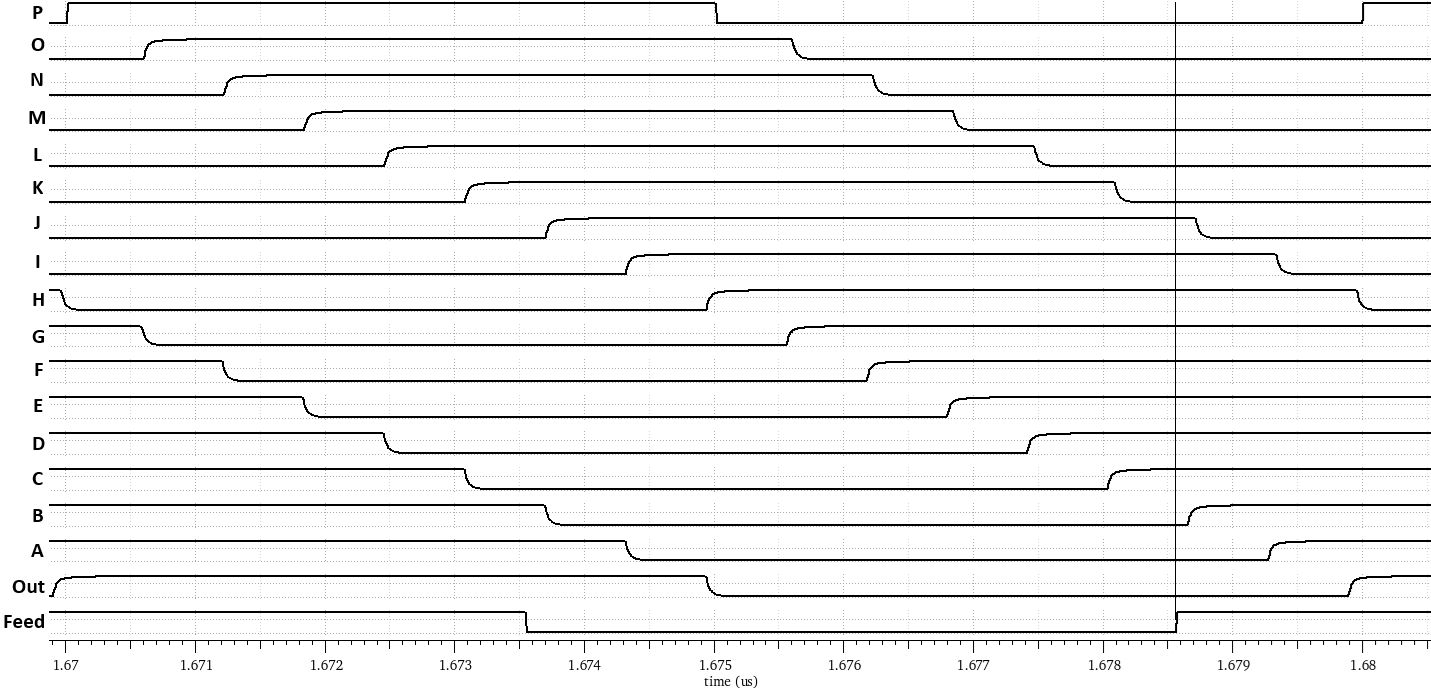
\includegraphics[width=1\textwidth]{figures/DLL_TRAN.png}
    \caption{Timing diagram of the DLL output.}
    \label{fig:DLL_output_TRAN}
\end{figure}

Two modifications are made to the decoder. First, each path of the TDC (forward and backward) has its own decoder. This is necessary to solve the issue of the 0 gain zone around zero delay
(see Fig. \ref{fig:TDC_conventional_timing_diagram}) and is achieved by making the forward decoder output a minimum value of 1 instead of 0 when the delay is small. Such a modification essentially shifts
the output characteristic (Fig. \ref{fig:TDC_shifted_characteristic}) of the TDC up by 1, eliminating the 0 gain zone.

\begin{figure}[H]
    \centering
    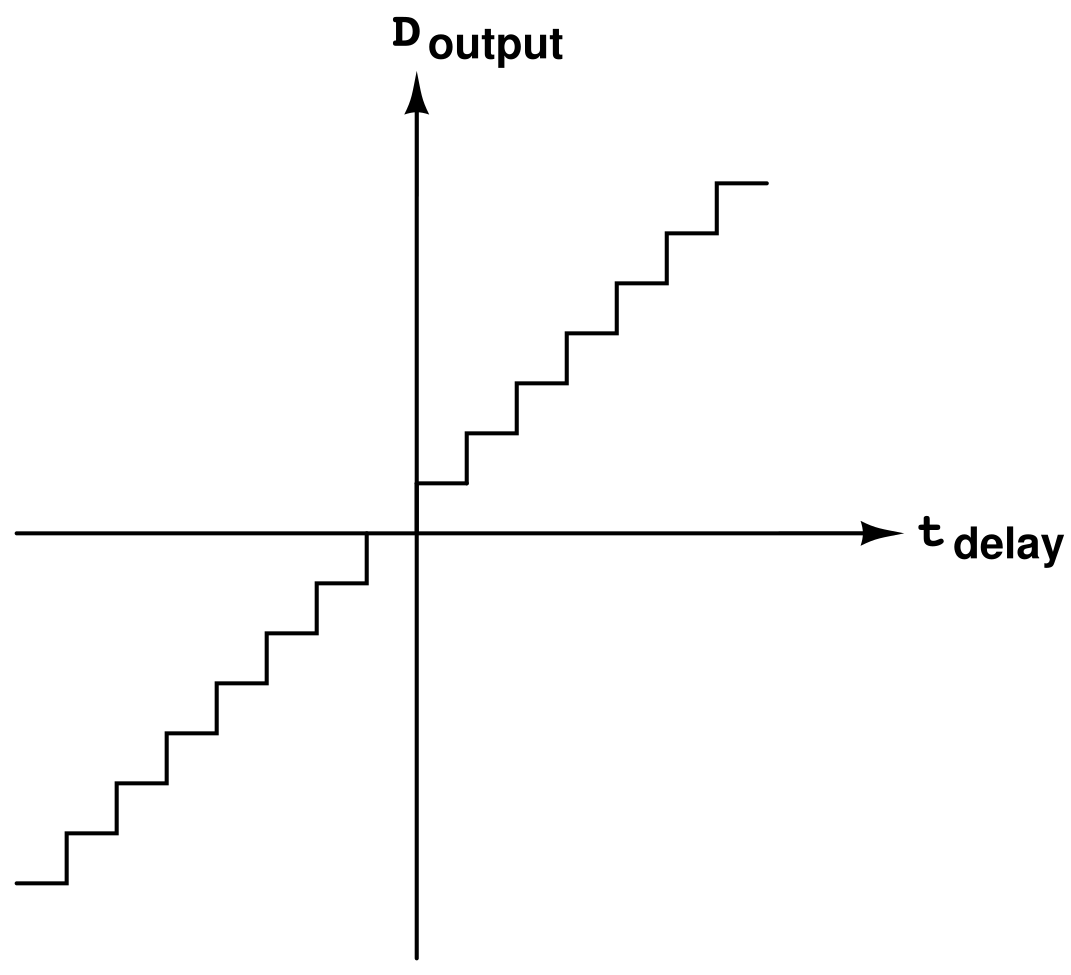
\includegraphics[width=0.6\textwidth]{figures/TDC_shifted_characteristic.png}
    \caption{Ideal characteristic of the TDC with the modified decoders.}
    \label{fig:TDC_shifted_characteristic}
\end{figure}

The second modification is what allows the TDC to read a phase difference of $\pm2\pi$ each cycle. The modified truth tables for the forward and backward decoders are shown in tables
\ref{tab:fwd_truth_table} and \ref{tab:bwd_truth_table} respectively. 

\begin{minipage}
{0.48\textwidth}
    \centering
    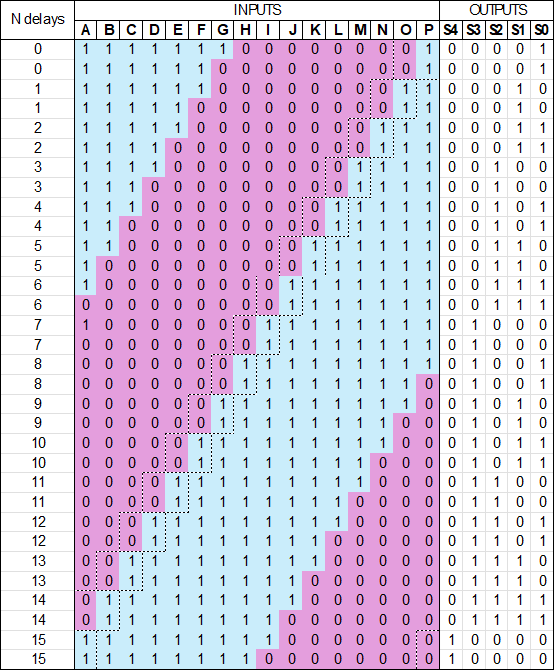
\includegraphics[width=1.04\textwidth]{figures/fwd_truth_table.png}
    \captionof{table}{Truth table of the modified forward thermometer-to-binary decoder for a 4-bit TDC.}
    \label{tab:fwd_truth_table}
\end{minipage}
\hspace{0.02\textwidth}
\begin{minipage}{0.48\textwidth}
    \centering
    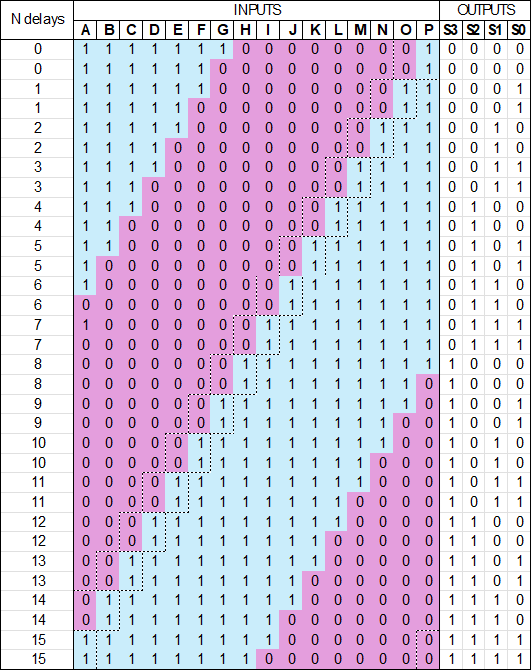
\includegraphics[width=1\textwidth]{figures/bwd_truth_table.png}
    \captionof{table}{Truth table of the modified backward thermometer-to-binary decoder for a 4-bit TDC.}
    \label{tab:bwd_truth_table}
\end{minipage}

Recognizing that the only two conditions defining each output of both decoders are the high state of its decimal equivalent DLL output (e.g L=high for the number 4 in decimal) and the low state of the next number
(e.g K=low), it is possible to obtain the bool equations for this otherwise large truth tables. The set of bool equations for the forward decoder are shown in \ref{eq:fwd_decoder_bool_eqs}, while those for
the backward decoder are shown in \ref{eq:bwd_decoder_bool_eqs}.

\begin{equation}
    \begin{aligned}
        S_0 &= A\overline{B} + C\overline{D} + E\overline{F} + G\overline{H} + I\overline{J} + K\overline{L} + M\overline{N} + O\overline{P} \\
        S_1 &= A\overline{B} + B\overline{C} + E\overline{F} + F\overline{G} + I\overline{J} + J\overline{K} + M\overline{N} + N\overline{O}\\
        S_2 &= A\overline{B} + B\overline{C} + C\overline{D} + D\overline{E} + I\overline{J} + J\overline{K} + K\overline{L} + L\overline{M}\\
        S_3 &= A\overline{B} + B\overline{C} + C\overline{D} + D\overline{E} + E\overline{F} + F\overline{G} + G\overline{H} + H\overline{I}\\
        S_4 &= A\overline{P}\\
    \end{aligned}
    \label{eq:fwd_decoder_bool_eqs}
\end{equation}

\begin{equation}
    \begin{aligned}
        S_0 &= (O + \overline{P}) (B\overline{C} + D\overline{E} + F\overline{G} + H\overline{I} + J\overline{K} + L\overline{M} + N\overline{O} + A\overline{P})\\
        S_1 &= (O + \overline{P}) (A\overline{B} + D\overline{E} + E\overline{F} + H\overline{I} + I\overline{J} + L\overline{M} + M\overline{N} + A\overline{P})\\
        S_2 &= (O + \overline{P}) (A\overline{B} + B\overline{C} + C\overline{D} + H\overline{I} + I\overline{J} + J\overline{K} + K\overline{L} + A\overline{P})\\
        S_3 &= (O + \overline{P}) (A\overline{B} + B\overline{C} + C\overline{D} + D\overline{E} + E\overline{F} + F\overline{G} + G\overline{H} + A\overline{P})\\
    \end{aligned}
    \label{eq:bwd_decoder_bool_eqs}
\end{equation}

\subsubsection{PFD selector circuit}
Because of the modifications done to the decoders, the TDC is now able to read a phase difference of $\pm2\pi$ each cycle, but it has lost the ability to determine whether the feedback signal is leading or lagging
the reference clock. This information is necessary for the PLL to be able to correct the phase difference, therefore a circuit that retrieves this information is needed. The approach taken in this work is to use
another PFD identical to the one of the DLL but with additional circuitry to determine whether the feedback signal is leading or lagging.

Figure \ref{fig:PFD_selector} shows the schematic of the PFD selector circuit. The additional circuitry consists of two AND and two NOT gates that process the UP and DOWN signals of the PFD and eliminate the
glitches that occur when both signals are high. The resulting signals are then used as the set and reset inputs of a SR latch, whose output (Q) indicates whether the feedback signal is leading or lagging the
reference clock.

\begin{figure}[H]
    \centering
    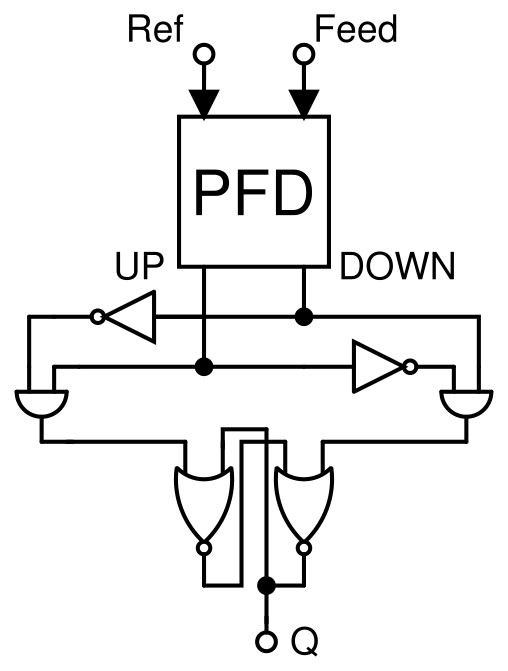
\includegraphics[width=0.4\textwidth]{figures/PFD_selector.png}
    \caption{PFD selector circuit schematic.}
    \label{fig:PFD_selector}
\end{figure}

\subsubsection{Adder}
The adder is only necessary for the backward path of the TDC, as it needs to do the 2's complement of the backward decoder output before it is sent to the multiplexer. however, because this block adds a significant 
amount of delay to the backward path, it is also added to the forward path (only adding zeros) to balance the delays of both paths.

The adder is implemented using a carry look-ahead (CLA) architecture to minimize the delay as much as possible. Because the forward path has an extra bit (S$_4$) that the backward path doesn't have, the adder is a
5-bit adder for both cases.

\subsubsection{multiplexer}
The multiplexer is a simple 2-to-1 multiplexer that selects between the outputs of the forward and backward decoders based on equation \ref{eq:MUX_equation} and according to the output of the PFD selector circuit.
If Q=1, then the feedback signal is lagging the reference clock and the output of the TDC is that of the forward decoder.                                                                                                                                                                                                                                                                                                                                                                                                                                                                                                                                                                                                                                                                                                                                                                                                                                                                                                                                                                                                                                                                                                                                                                                                                                                                                                                                                                                                                                                                                                                                                                                                                                                                                                                                                                                                                                                                                                                                                                                                                                                                                                                                                                                                                                                                                                                                                                                                                                                                                                                                                                                                                                                                                                                                                                                                                                                                                                                                                                                                                                                                                                                                                                                                                                                                                                                                                                                                                                                                                                                                                                                                                                                                                                                                                                                                                                                                                                                                                                                                                                                                                                                                                                                                                                                                                                                                                                                                                                                                                                                                                                                                                                                                                                                                                                                                                                                                                                                                                                                                                                                                                                                                                                                                                                                                                                                                                                                                                                                                                                                                                                                                                                                                                                                                                                                                                                                                                                                                                                                                                                                                                                                                                                                                                                                                                                                                                                                                                                                                                                                                                                                                                                                                                                                                                                                                                                                                                                                                                                                                                                                                                                                                                                                                                                                                                                                                                                                                                                                                                                                                                                                                                                                                                                                                                                                                                                                                                                                                                                                                                                                                                                                                                                                                                                                                                                                                                                                                                                                                                                                                                                                                                                                                                                                                                                                                                                                                                                                                                                                                                                                                                                                                                                                                                                                                                                                                                                                                                                                                                                                                                                                                                                                                                                                                                                                                                                                                                                                                                                                                                                                                                                                                                                                                                                                                                                                                                                                                                                                                                                                                                                                                                                                                                                                                                                                                                                                                                                                                                                                                                                                                                                                                                                                                                                                                                                                                                                                                                                                                                                                                                                                                                                                                                                                                                                                                                                                                                                                                                                                                                                                                                                                                                                                                                                                                                                                                                                                                                                                                                                                                                                                                                                                                                                                                                                                                                                                                                                                                                                                                                                                                                                                                                                                                                                                                                                                                                                                                                                                                                                                                                                                                                                                                                                                                                                                                                                                                                                                                                                                                                                                                                                                                                                                                                                                                                                                                                                                                                                                                                                                                                                                                                                                                                                                                                                                                                                                                                                                                                                                                                                                                                                                                                                                                                                                                                                                                                                                                                                                                                                                                                                                                                                                                                                                                                                                                                                                                                                                                                                                                                                                                                                                                                                                                                                                                                                                                                                                                                                                                                                                                                                                                                                                                                                                                                                                                                                                                                                                                                                                                                                                                                                                                                                                                                                                                                                                                                                                                                                                                                                                                                                                                                                                                                                                                                                                                                                                                                                                                                                                                                                                                                                                                                                                                                                                                                                                                                                                                                                                                                                                                                                                                                                                                                                                                                                                                                                                                                                                                                                                                                                                                                                                                                                                                                                                                                                                                                                                                                                                                                                                                                                                                                                                                                                                                                                                                                                                                                                                                                                                                                                                                                                                                                                                                                                                                                                                                                                                                                                                                                                                                                                                                                                                                                                                                                                                                                                                                                                                                                                                                                                                                                                                                                                                                                                                                                                                                                                                                                                                                                                                                                                                                                                                                                                                                                                                                                             If Q=0, then the feedback signal is leading the reference clock and the output of the TDC
is that of the backward decoder. 

\begin{equation}
    \text{TDC}_{n} = Q \cdot \text{FWD}_{n} + \overline{Q} \cdot \text{BWD}_{n}
    \label{eq:MUX_equation}
\end{equation}

\section{Digitally controlled oscillator}
The digitally controlled oscillator (DCO) is implemented using an NMOS cross-coupled pair with an LC tank load. The frequency control is done by switching in and out different branches with binary weighted capacitors.
The implementation of the DCO is shown in figure \ref{fig:DCO_implementation}.

\begin{figure}[H]
    \centering
    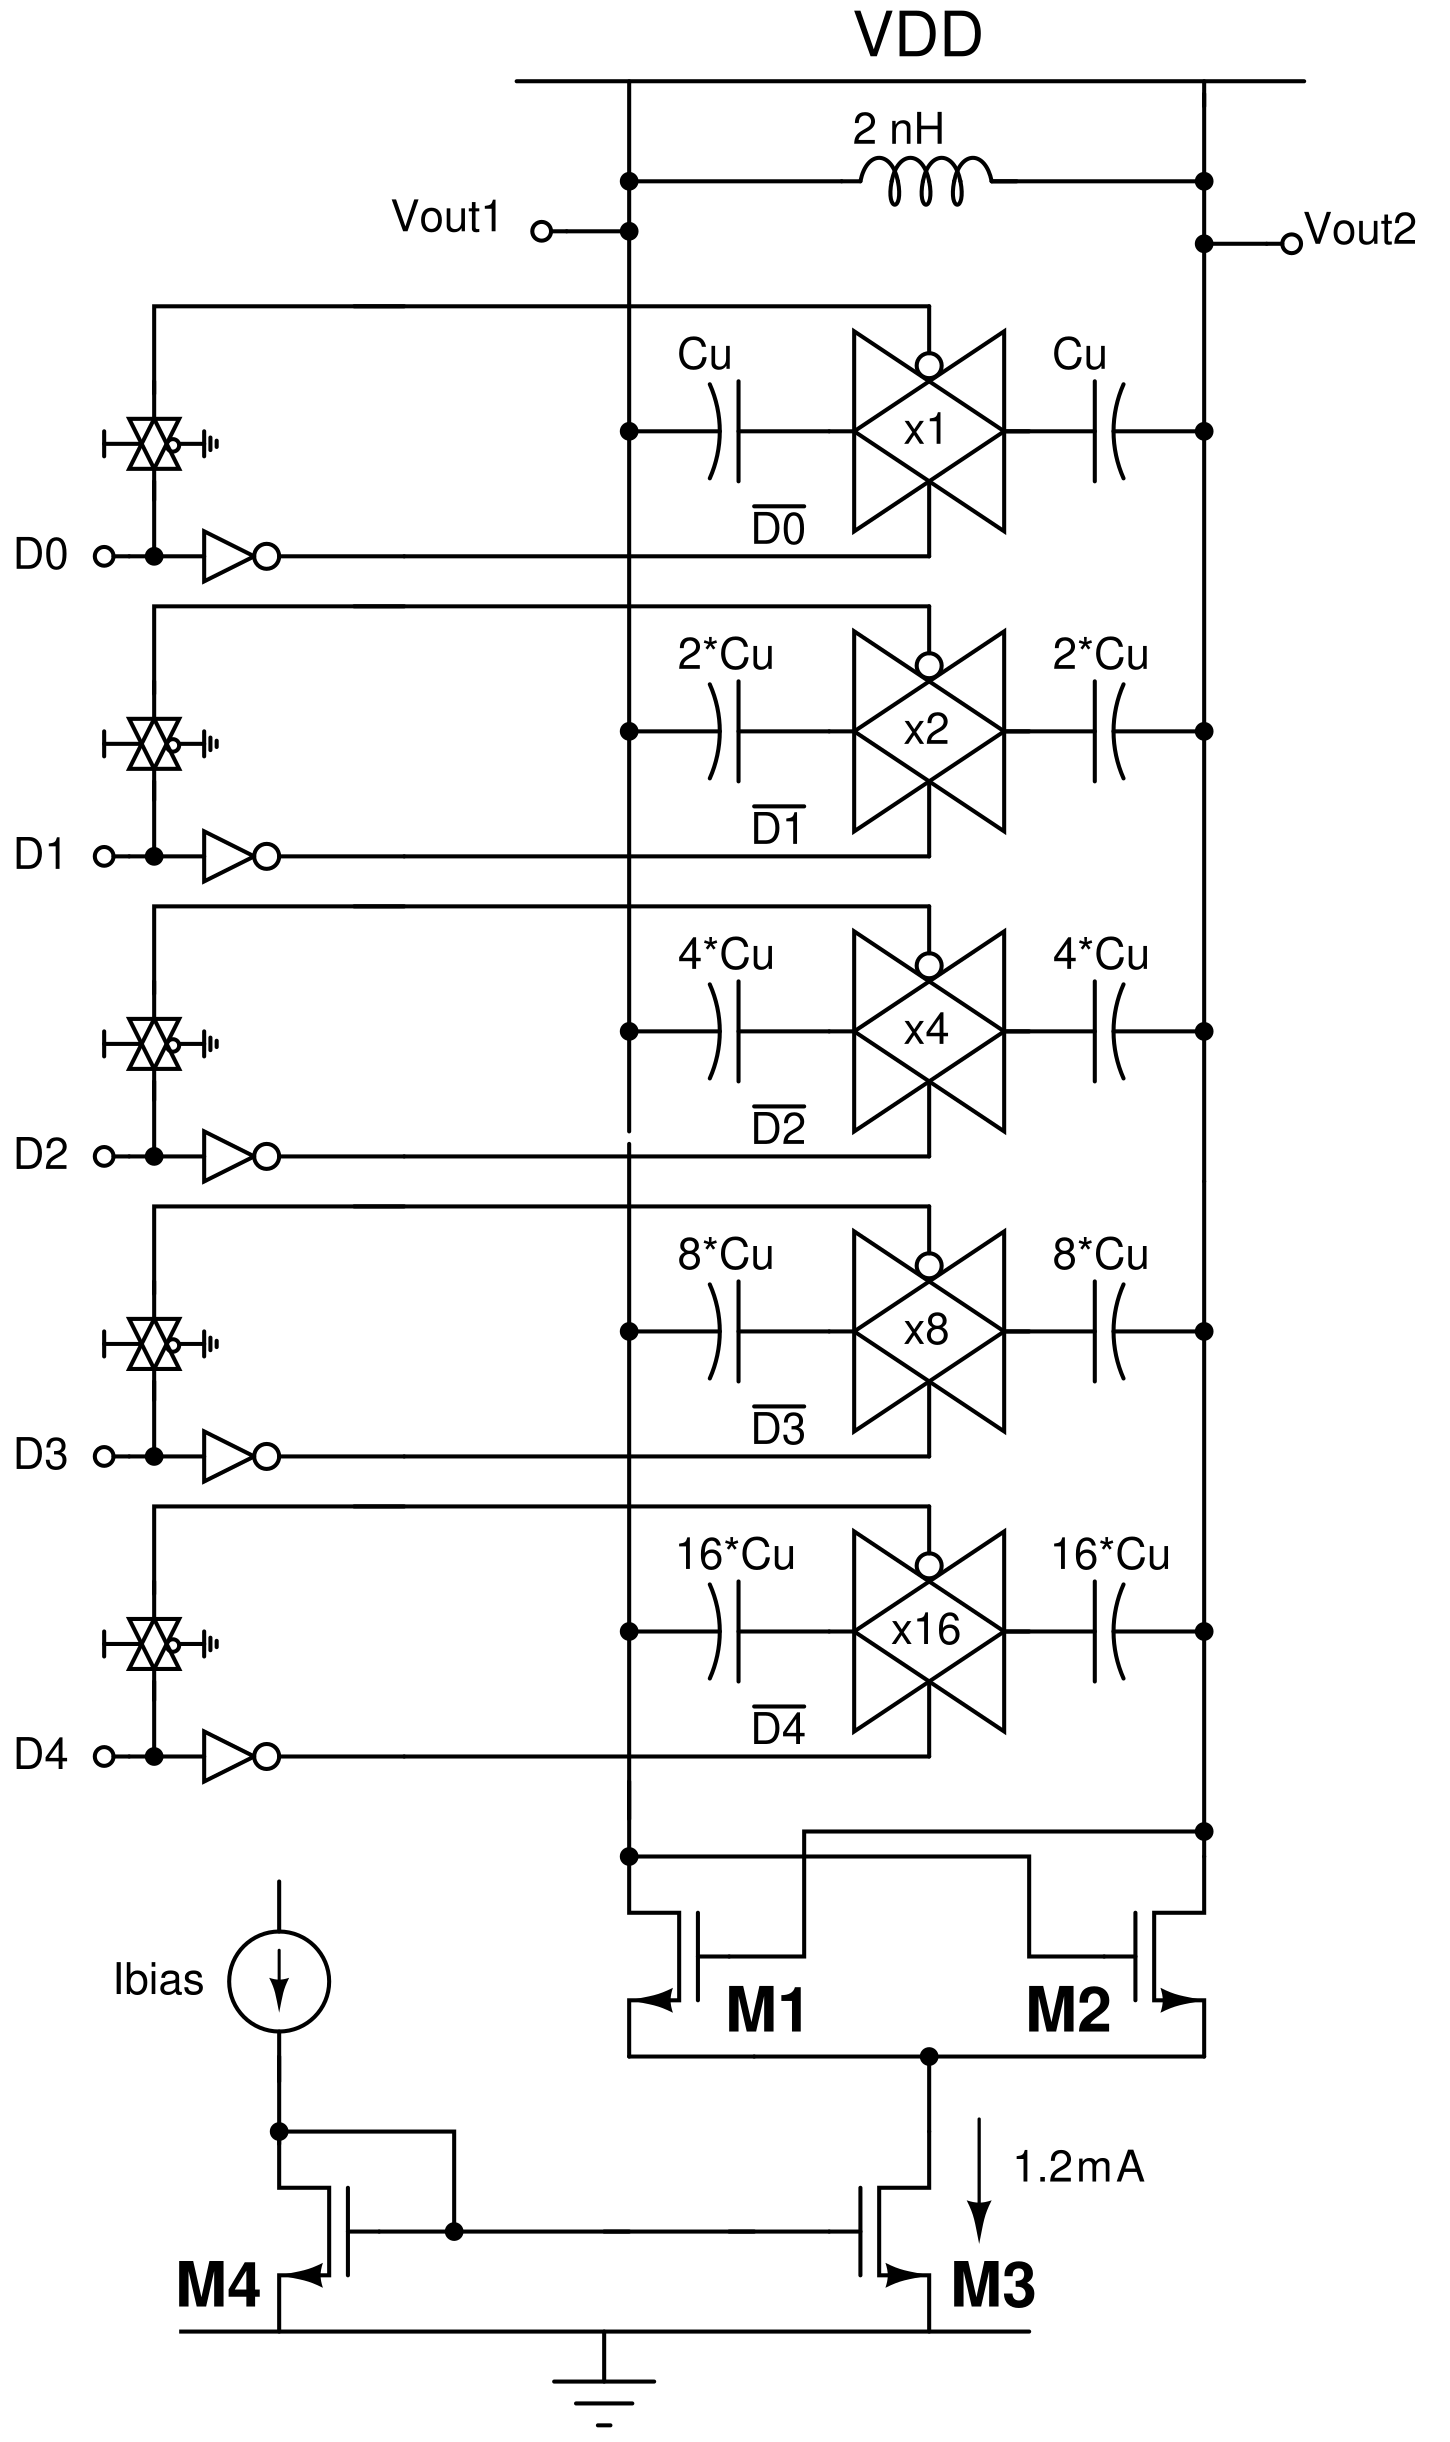
\includegraphics[width=0.6\textwidth]{figures/DCO_implementation.png}
    \caption{DCO implementation schematic.}
    \label{fig:DCO_implementation}
\end{figure}

Notice that there are CMOS inverters between the output of the digital loop filter and the DCO, this is done because the frequency of oscillation of the DCO decreases when the control voltage increases (adding 
capacitance) and it should be the opposite, otherwise the loop of the PLL would have positive feedback.

\subsection{System behavior}


\subsection{Specifications}
The specifications for the DCO are the following:
\begin{itemize}
    \item Corner set up: TT, 60$^{\circ}$C, 1.2 V.
    \item Center frequency: 8 GHz.
    \item Tuning range: 7.5 GHz to 8.5 GHz.
    \item Number of bits: 5.
    \item Frequency resolution: ~31.25 MHz.
    \item Phase noise: < -80 dBc/Hz at 100 kHz offset from the carrier.
    \item Tail current = 5 mA.
\end{itemize}
All of the above specifications are set to be met at the nominal corner considering a layout routing parasitic contribution of 50 fF (so a proper layout for this design should have equal or less capacitance). 


\subsection{Design process}
The design of the DCO is based on the LC resonator, which natural frequency of oscillation is given by equation \eqref{eq:LC_tank_frequency}. In order to correctly design the DCO, it is
first necessary to characterize the inductor to know its parasitic series resistance and its quality factor (Q). Once both parameters are known, the equivalent parallel resistance (R$_p$) can
be calculated with equation \eqref{eq:cross_coupled_pair_equation} to give dimensions to the cross-coupled pair. After that, the capacitor array can be designed. This procedure is explained in detail below.

\subsubsection{Inductor}
The inductor's Q is related to its equivalent parallel resistance (R$_p$) and can be approximated as $L\omega Q$. Considering the worst case for R$_p$ (at the minimum frequency of the tuning range)
and setting the inductance to 2 nH yields a Q of 13.3 for the inductor model used ($L\_SYCT30K\_RFVIL$). Equation \eqref{eq:Rp} is the constraint that will determine the cross-coupled dimensions in this design.


\begin{equation}
    Rp = L \omega Q = 2 \pi \cdot 2 x 10^{-9} \cdot 7.5 x 10^{9} \cdot 13.3 = 1.17 k \Omega
    \label{eq:Rp}
\end{equation}


The inductor also has parasitic capacitance in parallel, this model adds approximately 38.66 fF at the resonant frequency (18.1 GHz) and shall be taken into account for an accurate design.

\subsubsection{Cross-coupled pair}

In order to compensate for the inductor losses and sustain oscillation, the negative resistance generated by the cross-coupled pair must be much less than 1.17 k$\Omega$. The minimum transconductance necessary
to achieve such a resistance is therefore 1.71 mS according to \eqref{eq:cross_coupled_pair_equation}, but it will be designed to be 10 times bigger at 17.1 mS. The dimensions needed to achieve that \textit{gm}
are L = 120 nm and W = 9 $\mu$m.

By doing the small signal analysis of the circuit it can be shown that the cross-coupled pair adds an additional capacitance in parallel to the inductor and its value is given by equation \eqref{eq:pair_parasitic_cap}.
Only the gate-drain capacitance ($C_{gd}$) and the gate-source capacitance ($C_{gs}$) are considered for this analysis.

\begin{equation}
    C_{pair} = \frac{1}{3} W L \cdot C_{ox} + \frac{5}{2} C_{ov} W 
    \label{eq:pair_parasitic_cap}
\end{equation}

Where C$_{ox}$ is the oxide capacitance per unit area (13.275 fF/$\mu^2$ for this technology) and C$_{ov}$ is the overlap capacitance per unit width (0.212 fF/$\mu^2$).

Notice that the previous analysis assumes that the cross-coupled pair is perfectly matched and at the zero common-mode output voltage point to take into account the worst case for the noise performance.

For this design the cross-coupled pair adds an additional 9.55 fF in parallel with the inductor.

\subsubsection{Capacitor array}
The capacitor array is the method used to control the frequency of oscillation, turning on or off the branches containing the binary weighted capacitors to either increase or decrease the output frequency. Each
branch connecting both output nodes of the DCO is composed of 2 identical capacitors in series with a bidirectional switch between them, the values of such capacitors are binary weighted multiples of a unit capacitor
($C_u$) like in the schematic of figure \ref{fig:DCO_implementation}.

The unit capacitance is designed to be 9 fF, so accounting for all five branches there is a total of 558 fF in the array, though this is not the load in parallel with the inductor even if all branches are
switched on. The analysis for both cases (either switched on or off) is done below.

\subsubsection{Switches}
The switches themselves add parasitic capacitance to the circuit,depending on whether theyre are turned on or off. Figure \ref{fig:DCO_switches} a) shows the equivalent circuit of a single branch in figure
\ref{fig:DCO_implementation} for the case in which the switch is turned on, while figure \ref{fig:DCO_switches} b) shows the case for which the switched is turned off.


\begin{figure}[H]
    \centering
    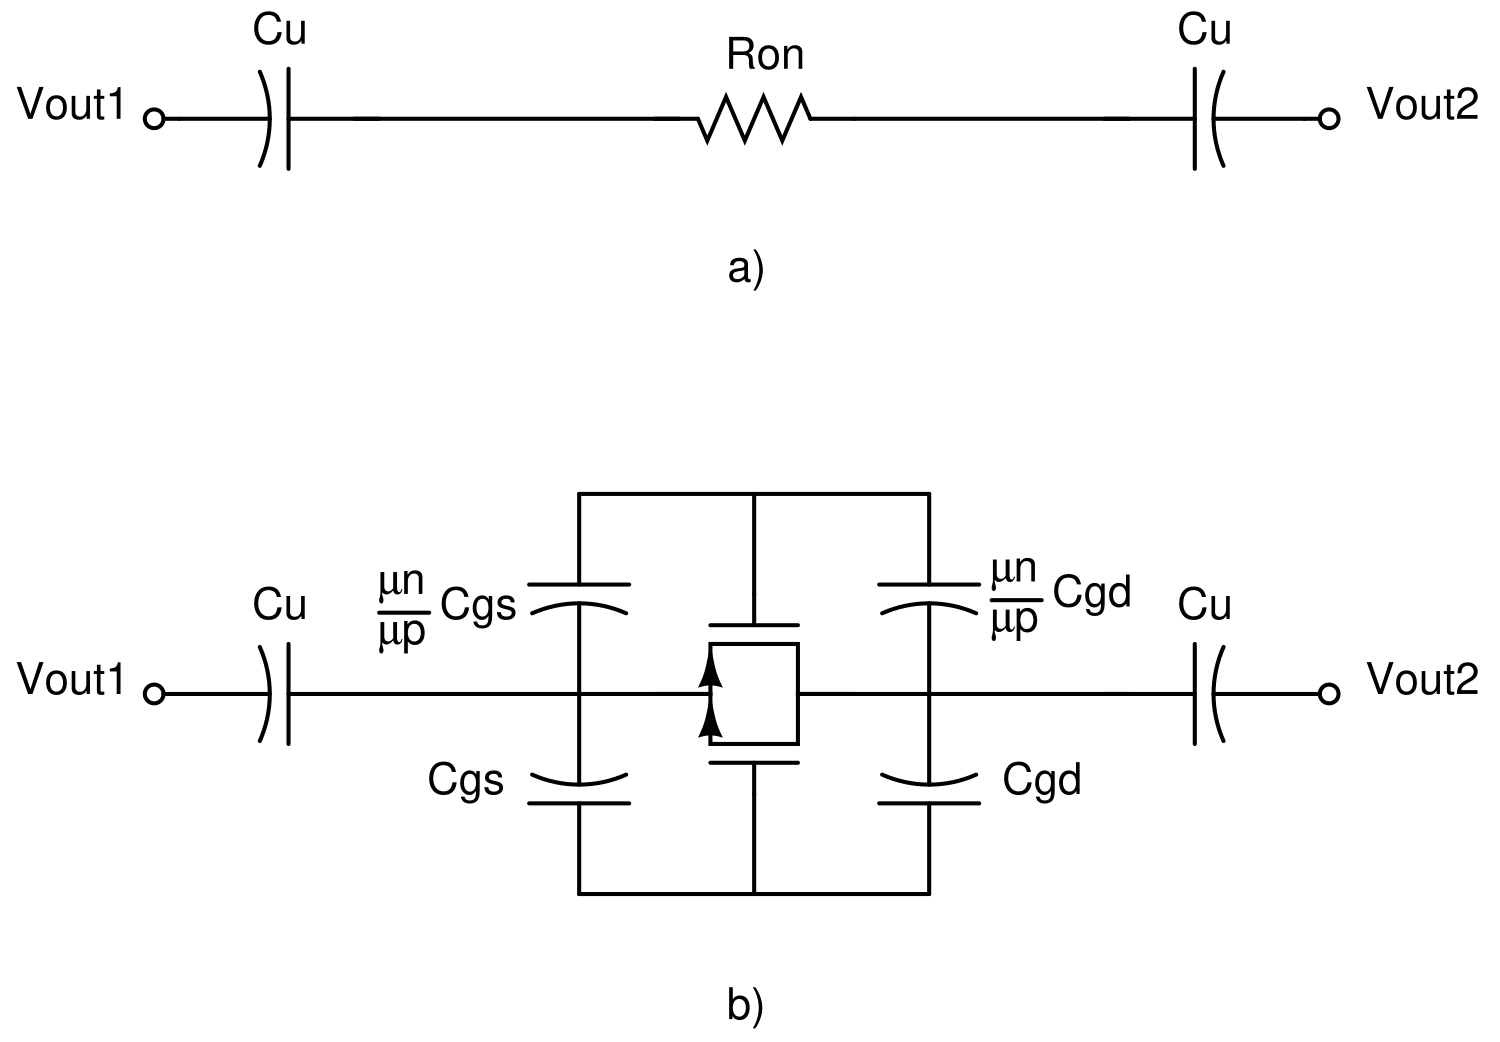
\includegraphics[width=0.6\textwidth]{figures/DCO_switches.png}
    \caption{Capacitor array branch: a) turned-on and b) turned-off}
    \label{fig:DCO_switches}
\end{figure}

If the switches are designed in such a way that the on-resistance can be assumed to be negligible, then an approximation can be made for the equivalent capacitance of each branch for the case in which the switch
is on. This is shown in equation \eqref{eq:branch_on}, where the equivalent capacitance of each branch per unit capacitor is half the value of the unit capacitor ($C_u$) itself. Therefore, if all branches are 
turned on, the total capacitance of the array is 139.5 fF. If the analysis is done for the case in which the switches are turned off, then the equivalent capacitance per unit capacitor is dominated by the parasitic
capacitances of the NMOS and the PMOS, so assuming $C_{gs} = C_{gd}$ and that the PMOS device is 2.5 times wider than the NMOS the expression for the off case is given by equation \eqref{eq:branch_off}.

\begin{equation}
    C_{on} \approx \frac{C_u}{2}
    \label{eq:branch_on}
\end{equation}

\begin{equation}
    C_{off} \approx 1.75 \cdot C_{gs, NMOS}
    \label{eq:branch_off}
\end{equation}

\subsubsection{Summary}

Table \ref{tab:DCO_capacitance_contribution} is a summary of all the different capacitance contributions for the DCO as well as its estimated frequency range ($f_{max} \, \& \, f_{min}$). Table \ref{tab:DCO_dimensions}
shows the dimensions of all the transistors used in the DCO design.

\begin{table}[H]
    \centering
    \caption{DCO capacitance contributions.}
    \begin{tabular}{|c|c|c|}
        \hline
        Contribution & Capacitance (fF) & Frequency (GHz) \\
        \hline
        Inductor parasitic & 38.66 & - \\
        Cross-coupled pair parasitic & 9.55 & - \\
        Capacitor array (all on) & 139.5 & - \\
        Capacitor array (all off) & 67.44 & - \\
        Routing parasitic & 50 & - \\
        \hline
        Total (all on) & 237.71 & 7.3 \\
        Total (all off) & 165.65 & 8.74 \\
        \hline
    \end{tabular}
    \label{tab:DCO_capacitance_contribution}
\end{table}

\begin{table}[H]
    \centering
    \caption{DCO transistor dimensions.}
    \begin{tabular}{|c|c|c|}
        \hline
        Transistor & L (nm) & W ($\mu$m) \\
        \hline
        M1, M2 (cross-coupled pair) & 120 & 9 \\
        M3 (tail current source) & 300 & 100 \\
        M4 (biasing diode) & 300 & 12.5 \\
        NMOS switch (unitary) & 120 & 5.5 \\
        PMOS switch (unitary) & 120 & 13 \\
        \hline
    \end{tabular}
    \label{tab:DCO_dimensions}
\end{table}

%\section{Digital loop filter}

\noindent\rule{\textwidth}{1pt}